\documentclass[NormeDiProgetto.tex]{subfiles}

\begin{document}
	
	\chapter{Processi di supporto}
	
	\section{Documentazione}
	\subsection{Descrizione}
	Questo capitolo descrive le scelte intraprese per la
	stesura, \citGloss{verifica} e approvazione riguardante la documentazione ufficiale.
	Tali norme sono tassative per tutti i documenti formali.
	Tali documenti sono elencati successivamente nella sotto-sezione \textquotedblleft Documenti correnti\textquotedblright. 
	
	\subsection{Ciclo di vita documentazione}
	Ogni documento formale deve passare gli stadi di \textquotedblleft Sviluppo\textquotedblright, \textquotedblleft Verifica\textquotedblright e \textquotedblleft Approvato\textquotedblright.
	\begin{itemize}
		\item \textbf{Sviluppo:} inizia con la creazione del documento e termina con la conclusione della stesura di tutte le sue parti. In questa fase i Redattori aggiungono le parti assegnate tramite \citGloss{ticket}.
		Il passaggio alla fase di \citGloss{verifica} è automatizzato con la segnalazione al Responsabile;
		
		\item \textbf{Verifica:} il documento entra nella fase di verifica dopo l'assegnazione da parte del Responsabile. I Verificatori effettueranno le procedure di controllo dello stesso.\\
		Al termine del controllo in caso positivo il documento entra automaticamente in fase di \textquotedblleft Approvato\textquotedblright, altrimenti i loro riscontri vengono consegnati al Responsabile di Progetto, che provvederà ad assegnare nuovamente il documento ad un Redattore attraverso una nuova fase di Sviluppo; 
		
		\item \textbf{Approvato:} l'approvazione di un documento coincide con il superamento positivo da parte di un verificatore dello stadio di \citGloss{verifica} comunicato al Responsabile che approva il documento per il rilascio esterno.
	\end{itemize}
	
	\subsection{Separazione documenti interni ed esterni}
	Ogni documento formale dovrà essere classificato come Interno
	oppure Esterno con le seguenti differenze:
	\begin{itemize}
		\item \textbf{Interno:} ha utilizzo interno al gruppo \gruppo, redatto in lingua Italiana;
		\item \textbf{Esterno:} verrà condiviso con la Proponente ed i committenti, nel caso sia utile per il deploy dell'applicazione web o per il suo utilizzo da parte degli utenti finali, dovrà essere redatto in lingua Inglese.
	\end{itemize}
	Un documento formale farà sempre parte di una delle due categorie elencate.
	
	\subsection{Nomenclatura documenti}
	Tutti i documenti formali tranne Verbali e Lettera di Presentazione seguiranno questo sistema di nomenclatura:

	\begin{itemize}
		\item\textbf{NomeDocumento:} indica il nome del documento senza spazi e lettere maiuscole all'inizio di ogni parola;
		\item \textbf{vX.Y.Z:} indica il numero di versionamento con X,Y e Z numeri interi e non negativi.	
	\end{itemize}
	Di seguito la spiegazione che assumono le versione del documento:
	\begin{itemize}
		\item \textbf{X:} rappresenta il numero di pubblicazioni ufficiali del documento: ogni qual volta il documento viene pubblicato il valore di Y e Z viene azzerato, quello di X incrementato di uno;
		\item \textbf{Y:} rappresenta il numero di verifiche completate con successo, in caso di mancato superamento della fase di \citGloss{verifica} il valore non va modificato, mentre se superata viene incrementato di uno e si azzera il valore della Z;
		\item \textbf{Z:} rappresenta il numero di modifiche effettuate al documento durante il suo sviluppo.	
	\end{itemize}
	Formato dei file: ogni documento si trova nel formato .tex durante il suo ciclo di vita.
	Dopo lo stato di “Approvato” per il documento viene quindi creato un \citGloss{PDF} contenente la versione approvata dal Responsabile.
	
	\subsection{Documenti correnti}
	Qui di seguito si presentano i documenti formali in ordine alfabetico, classificati per appartenenza (Interno ed Esterno):
	\begin{itemize}
		\item \textbf{Analisi dei Requisiti:} utilizzo Esterno, sigla (AR) \\
		 Documento per esporre e scomporre i \citGloss{requisiti} del progetto contenente casi d'uso relativi al prodotto e diagrammi di interazione con l'utente. Gli Analisti lo scrivono dopo aver analizzato il capitolato e interagendo con il Proponente in riunioni esterne;
		
		\item \textbf{Glossario:}
		utilizzo Esterno, sigla (GL) \\
		Documento per raccogliere le definizioni dei termini o concetti che saranno usati nei documenti formali per facilitarne la comprensione;
		
		\item \textbf{Norme di Progetto:}
		utilizzo Interno, sigla (NdP) \\
		Documento per mostrare le direttive e gli standard utilizzati all'interno del gruppo di lavoro 353
		per lo sviluppo del progetto;
		
		\item \textbf{Piano di Progetto:}
		utilizzo Esterno, sigla (PdP) \\
		Documento per l'analisi e la pianificazione della gestione delle risorse di tempo e umane;
		
		\item \textbf{Piano di Qualifica:}
		utilizzo Esterno, sigla (PdQ) \\
		Documento per descrivere standard e obiettivi che il gruppo dovrà raggiungere per garantire la qualità di prodotto e processo;
		
		\item \textbf{Studio di Fattibilità:}
		utilizzo Interno, sigla (SdF) \\
		Documento per indicare le riflessioni, punti di forza e caratteristiche sfavorevoli per ogni capitolato che ha portato alla scelta finale del gruppo.
		
	\end{itemize}
	
	\subsection{Norme}
	\subsubsection{Struttura dei documenti}
		Ogni documento è realizzato a partire da una disposizione prestabilita che dovrà essere conforme per ogni documento ufficiale ad eccezione dei verbali e della lettera di presentazione:
		\begin{itemize}
			\item \textbf{Frontespizio:} questa sezione si troverà nella prima pagina di ogni documento e conterrà:
			\begin{itemize}
				\item Logo del gruppo;
				\item Titolo del documento;
				\item Versione del documento con l'ultima data di modifica;
				\item Nome del gruppo;
				\item Nome del progetto.
			\end{itemize}
			
			\item \textbf{Informazioni sul documento:} conterrà la lista di responsabili,
			redattori, verificatori del documento e infine lo stato e la tipologia di uso (vedi sotto sezione \textbf{Separazione documenti interni ed esterni});
			
			\item \textbf{Diario delle modifiche:}
			Questo diario sarà presente nella seconda pagina del documento sotto forma di tabella in ordine di versione decrescente con righe composte da: versione, data, descrizione modifiche, autore, ruolo;
			
			\item \textbf{Indice delle sezioni:}
			L'indice delle sezioni conterrà l'elenco di tutti gli argomenti trattati nel documento con la seguente struttura: titolo, argomento e numero pagina;
			
			\item \textbf{Indice delle tabelle:}
			Sezione contenente l'elenco delle tabelle con struttura identica all'indice delle sezioni;
			
			\item \textbf{Indice delle figure:}
			Sezione contenente l'elenco delle figure, immagini, grafici con struttura identica all'indice delle tabelle;
			
			\item \textbf{Introduzione:}
			scopo del documento, informazioni sul glossario e riferimenti utili sia normativi che informativi.
			 
			\item \textbf{Contenuto del documento:} il resto del documento è occupato dal contenuto.
			
			
		\end{itemize}
		
	\subsubsection{Norme tipografiche}
		\begin{itemize}
			\item \textbf{Intestazione} ogni pagina dopo frontespizio presenterà sulla sinistra il logo del gruppo e a destra il nome del capitolo corrente;
			
			\item \textbf{Piè pagina:} a sinistra è presente il nome del documento corrente con versione e a destra il numero di pagina; 
			
			\item \textbf{Virgolette:} alte singole ' ' per singolo carattere, alte doppie " " per racchiudere stringhe mentre quelle basse '\textless \textless ' '\textgreater \textgreater ' per racchiudere citazioni;
			 
			\item \textbf{Parentesi:} tonde per descrivere esempi e fornire sinonimi o precisazioni, quadre per rappresentare uno standard ISO, uno stato relativo a un \citGloss{ticket} o un riferimento ad un codice definito all'interno del documento stesso;
			
			\item \textbf{Punteggiatura:} ogni segno di punteggiatura deve essere seguito da uno spazio e non avere spazi precedenti al segno stesso;

			\item \textbf{Stile del testo:} 
			\begin{itemize}
				\item \textbf{Corsivo:} per dare enfasi ad una parola, un concetto o per indicare il nome di un tool/tecnologia;
				\item \textbf{Grassetto:} per i titoli, sottotitoli ed elementi di elenchi e liste;
				\item \textbf{Azzurro:} per indicare dei collegamenti ipertestuali.
			\end{itemize}
		
			\item \textbf{Elenchi:} ogni elenco avrà la prima parola di ogni elemento maiuscola seguita dal carattere 'due punti' (:) seguito dalla sua descrizione, mentre al termine dell'elemento si inserirà sempre il carattere 'punto e virgola' (;) tranne per l'ultimo elemento della lista per cui si userà il carattere 'punto' (.);
			 
			\item \textbf{Note a Piè pagina:} seguono le seguenti regole: 
			\begin{itemize}
				\item Devono presentare una numerazione progressiva all'interno del documento;
				\item Devono essere scritte solo una volta;
				\item Il primo carattere di ogni nota deve essere maiuscolo. Fanno eccezione i casi in cui la parola sia un acronimo oppure un link esterno.
			\end{itemize}
			 
			\item \textbf{Formati:}
			\begin{itemize}
				\item Date: scritte con lo standard DD-MM-YYYY dove YYYY indica l'anno, MM il mese e DD il giorno, inseribili nel formato corretto attraverso il comando \texttt{\textbackslash nData}. Per le date che servono a nominare i file dei verbali si utilizza invece il formato YYYY-MM-DD per averli in ordine cronologico esatto.
				\item Grassetto: lo stile grassetto va utilizzato per i titoli dei paragrafi e per i titoli degli elementi di un elenco; 
				\item URI: lo stile utilizzato per un URI è il corsivo di colore blu, in modo da mantenere una continuità con lo standard web attuale, utilizzabile col comando personalizzato \citGloss{LaTeX} \texttt{\textbackslash nURI}.
			\end{itemize}
			
			\item \textbf{Riferimenti informativi:}
			ogni riferimento a prodotti, software, guide, libri esterno al progetto deve essere indicato tramite un'annotazione a piè di pagina.			
			
			\item \textbf{Ruoli/Fasi/Revisioni di Progetto:} sono stati realizzati dei comandi personalizzati per poter richiamare la visualizzazione dei ruoli di progetto, per indicare le fasi e le revisioni di progetto secondo comandi unificati per tutti i documenti facilitando il lavoro dei Redattori.
			
			\item \textbf{Nomi:} sono stati realizzati dei comandi personalizzati per poter richiamare la visualizzazione dei seguenti termini:
			\begin{itemize}
				\item nome gruppo: \texttt{\textbackslash gruppo}, visualizza \textquotedblleft \gruppo\textquotedblright;
				\item nomi propri: \texttt{\textbackslash NomeProprioPersona};
				\item nome progetto: \texttt{\textbackslash progetto}, visualizza \textquotedblleft \progetto\textquotedblright;
				\item nome di un file: \texttt{\textbackslash nFile};
				\item nome di un documento: \texttt{\textbackslash nDoc};
				\item percorso cartelle: \texttt{\textbackslash nPath}.
			\end{itemize}
		
			\item \textbf{Componenti grafiche:}
			 \begin{itemize}
			 	\item \textbf{immagini:} i formati ammessi sono PNG o JPG inseriti tramite comando \texttt{\textbackslash nImg}; 
			 	\item \textbf{tabelle:} devono rispettare lo stile del template realizzato.
			 \end{itemize}
			
		\end{itemize}
	
	\subsection{Struttura documentazione}
	\`{E} stato creato un template di documento utilizzabile per tutti i documenti ufficiali in modo tale da favorire lo sviluppo dei documenti.\\
	Il template è basato sulle norme di documentazione elencate nella sezione precedente, inoltre è stata scritta una pagina dimostrativa di tutti i comandi personalizzati.
	
	\subsection{Gestione termini Glossario}
	Il glossario è un documento unico per tutti i documenti, esso conterrà tutte le definizioni, in ordine lessicografico crescente, dei termini inerenti al tema del progetto, che possono essere fraintesi o non ben comprensibili. I termini inseriti nel glossario saranno contrassegnati da una G pedice all'interno dei documenti.\\
	Ovviamente prima di inserire un nuovo termine bisognerà assicurarsi che non sia già presente, in modo da evitare duplicati. \\
	Il comando \LaTeX{} da utilizzare per contrassegnare un termine da glossario all'interno dei documenti è \texttt{\textbackslash{}citGloss}, mentre per l'inserimento di una nuova parola all'interno del glossario viene utilizzato \texttt{\textbackslash{}newglossaryentry }.\\
	La scelta di creare un comando apposito per una operazione \textquotedblleft elementare\textquotedblright\ è scaturita dall'agevolazione che porta alla stesura della documentazione: avendo un modo univoco di riconoscere i termini all'interno del glossario è stato possibile automatizzare la \citGloss{verifica} del soddisfacimento delle norme all'interno dei documenti tramite uno script denominato \textquotedblleft gupdate.sh\textquotedblright.\\
	In aggiunta è stato creato anche uno script denominato \textquotedblleft addterm.sh\textquotedblright\ che facilita l'inserimento di un termine all'interno del glossario.\\
	La descrizione dettagliata degli script è riposta nella sezione \textbf{Strumenti a supporto della documentazione}.
	
	
	\subsection{Ambiente}
	La stesura dei documenti deve essere effettuata utilizzando il linguaggio di markup \citGloss{LaTeX} e l'ambiente \citGloss{TexStudio}\footnote{\nURI{https://www.texstudio.org/}} con dizionario italiano ed inglese installati.
	
	\subsection{Strumenti di supporto alla documentazione}
	Per facilitare le attività di \citGloss{verifica} e manutenzione della documentazione, sono stati sviluppati degli script per automatizzare l'esecuzione di determinate attività. \\
	Tutti gli script sono eseguibili da qualsiasi distribuzione Linux, per i membri del gruppo che utilizzano Windows è richiesto il software Cygwin\footnote{\nURI{http://www.cygwin.com/}} oppure il Windows Subsystem for Linux\footnote{\nURI{https://en.wikipedia.org/wiki/Windows_Subsystem_for_Linux}}, per quanto riguarda i sistemi *BSD e macOS non è richiesto nessun programma aggiuntivo.\\
	In alcuni script sono richiesti dei programmi particolari, che vengono specificati, ove necessario, nell'elenco sottostante.
	\begin{itemize}
		\item \textbf{gupdate.sh [termine]:} si occupa di controllare le parole inserite nel glossario e, per ognuna di esse, aggiornare con il comando di glossario tutti i .tex file che le contengono. Se viene specificato un termine, lo script aggiorna solo quello indicato;
		\item \textbf{addterm.sh:} aggiunge un termine nel glossario ed esegue gupdate.sh per il termine appena inserito;
		\item \textbf{rmterm.sh [termine]:} rimuove un termine dal glossario e il corrispondente comando di glossario in tutte le occorrenze presenti nei file .tex;
		\item \textbf{compile.sh:} effettua la compilazione di tutti i file .tex presenti nelle sottocartelle, segnalando eventuali fallimenti;
		\item \textbf{build.sh:} esegue lo script compile.sh, aggiorna le occorrenze di glossario tramite gupdate.sh e compila nuovamente. In caso di errori durante il procedimento si blocca ed avvisa il suo esecutore. Questo script è necessario per l'approvazione del \citGloss{commit} da parte di \citGloss{Travis};
		\item \textbf{gulpease.py:} calcola l'indice di leggibilità Gulpease per tutti i documenti prodotti e mostra i risultati. Lo script, per essere eseguito, necessita dell'installazione di python\footnote{\nURI{https://www.python.org/}} (con versione minima richiesta 2.7) e del programma OpenDetex\footnote{\nURI{https://github.com/pkubowicz/opendetex}}.	
	\end{itemize}
	
	
	\section{Qualità}
	\subsection{Descrizione}
	Questa sezione descrive le classificazioni e procedure per il calcolo delle metriche descritte successivamente.
	\subsection{Classificazione dei processi}
	Per garantire la qualità del lavoro gli Amministratori hanno definito la divisone del lavoro in vari processi, che devono però rispettare la seguente notazione \textbf{PROC[num]}	dove:
	\begin{itemize}
		\item \textbf{num:} indica il codice univoco del processo come numero intero a tre cifre incrementale a partire da 1.
	\end{itemize}	
	
	\subsection{Classificazione delle metriche}
	Per garantire la qualità del lavoro gli Amministratori hanno definito delle metriche, che devono però rispettare la seguente notazione \textbf{M[categ][macrocateg][num]}	dove:
	\begin{itemize}
		\item \textbf{categ:} indica la categoria della metrica, può assume i valori:
		\begin{itemize}
			\item \textbf{PS:} per indicare i processi;
			\item \textbf{PD:} per indicare i prodotti;
			\item \textbf{TS:} per indicare i test.
		\end{itemize}
		\item \textbf{macrocateg:} indica la macro categoria della metrica, se esiste altrimenti non compare.\\
		Per le metriche di Prodotto \textbf{PD} può assumere i valori:
		\begin{itemize}
			\item \textbf{D:} per indicare i documenti;
			\item \textbf{S:} per indicare il software.
		\end{itemize}
		Per le metriche dei Test \textbf{TS} può assumere i valori:
		\begin{itemize}
			\item \textbf{A:} per indicare tutti i tipi di test;
			\item \textbf{M:} per indicare i test di modulo;
			\item \textbf{H:} per indicare i test ad alto livello.		
		\end{itemize}
		\item \textbf{num:} indica il codice univoco della metrica come numero intero a tre cifre incrementale a partire da 1.
	\end{itemize}	
	
	\subsection{Procedure}
	In questa fase del progetto, l'unica metrica che è stata implementata tramite procedura esterna è "MPDD001 - Indice di Gulpease":\\
	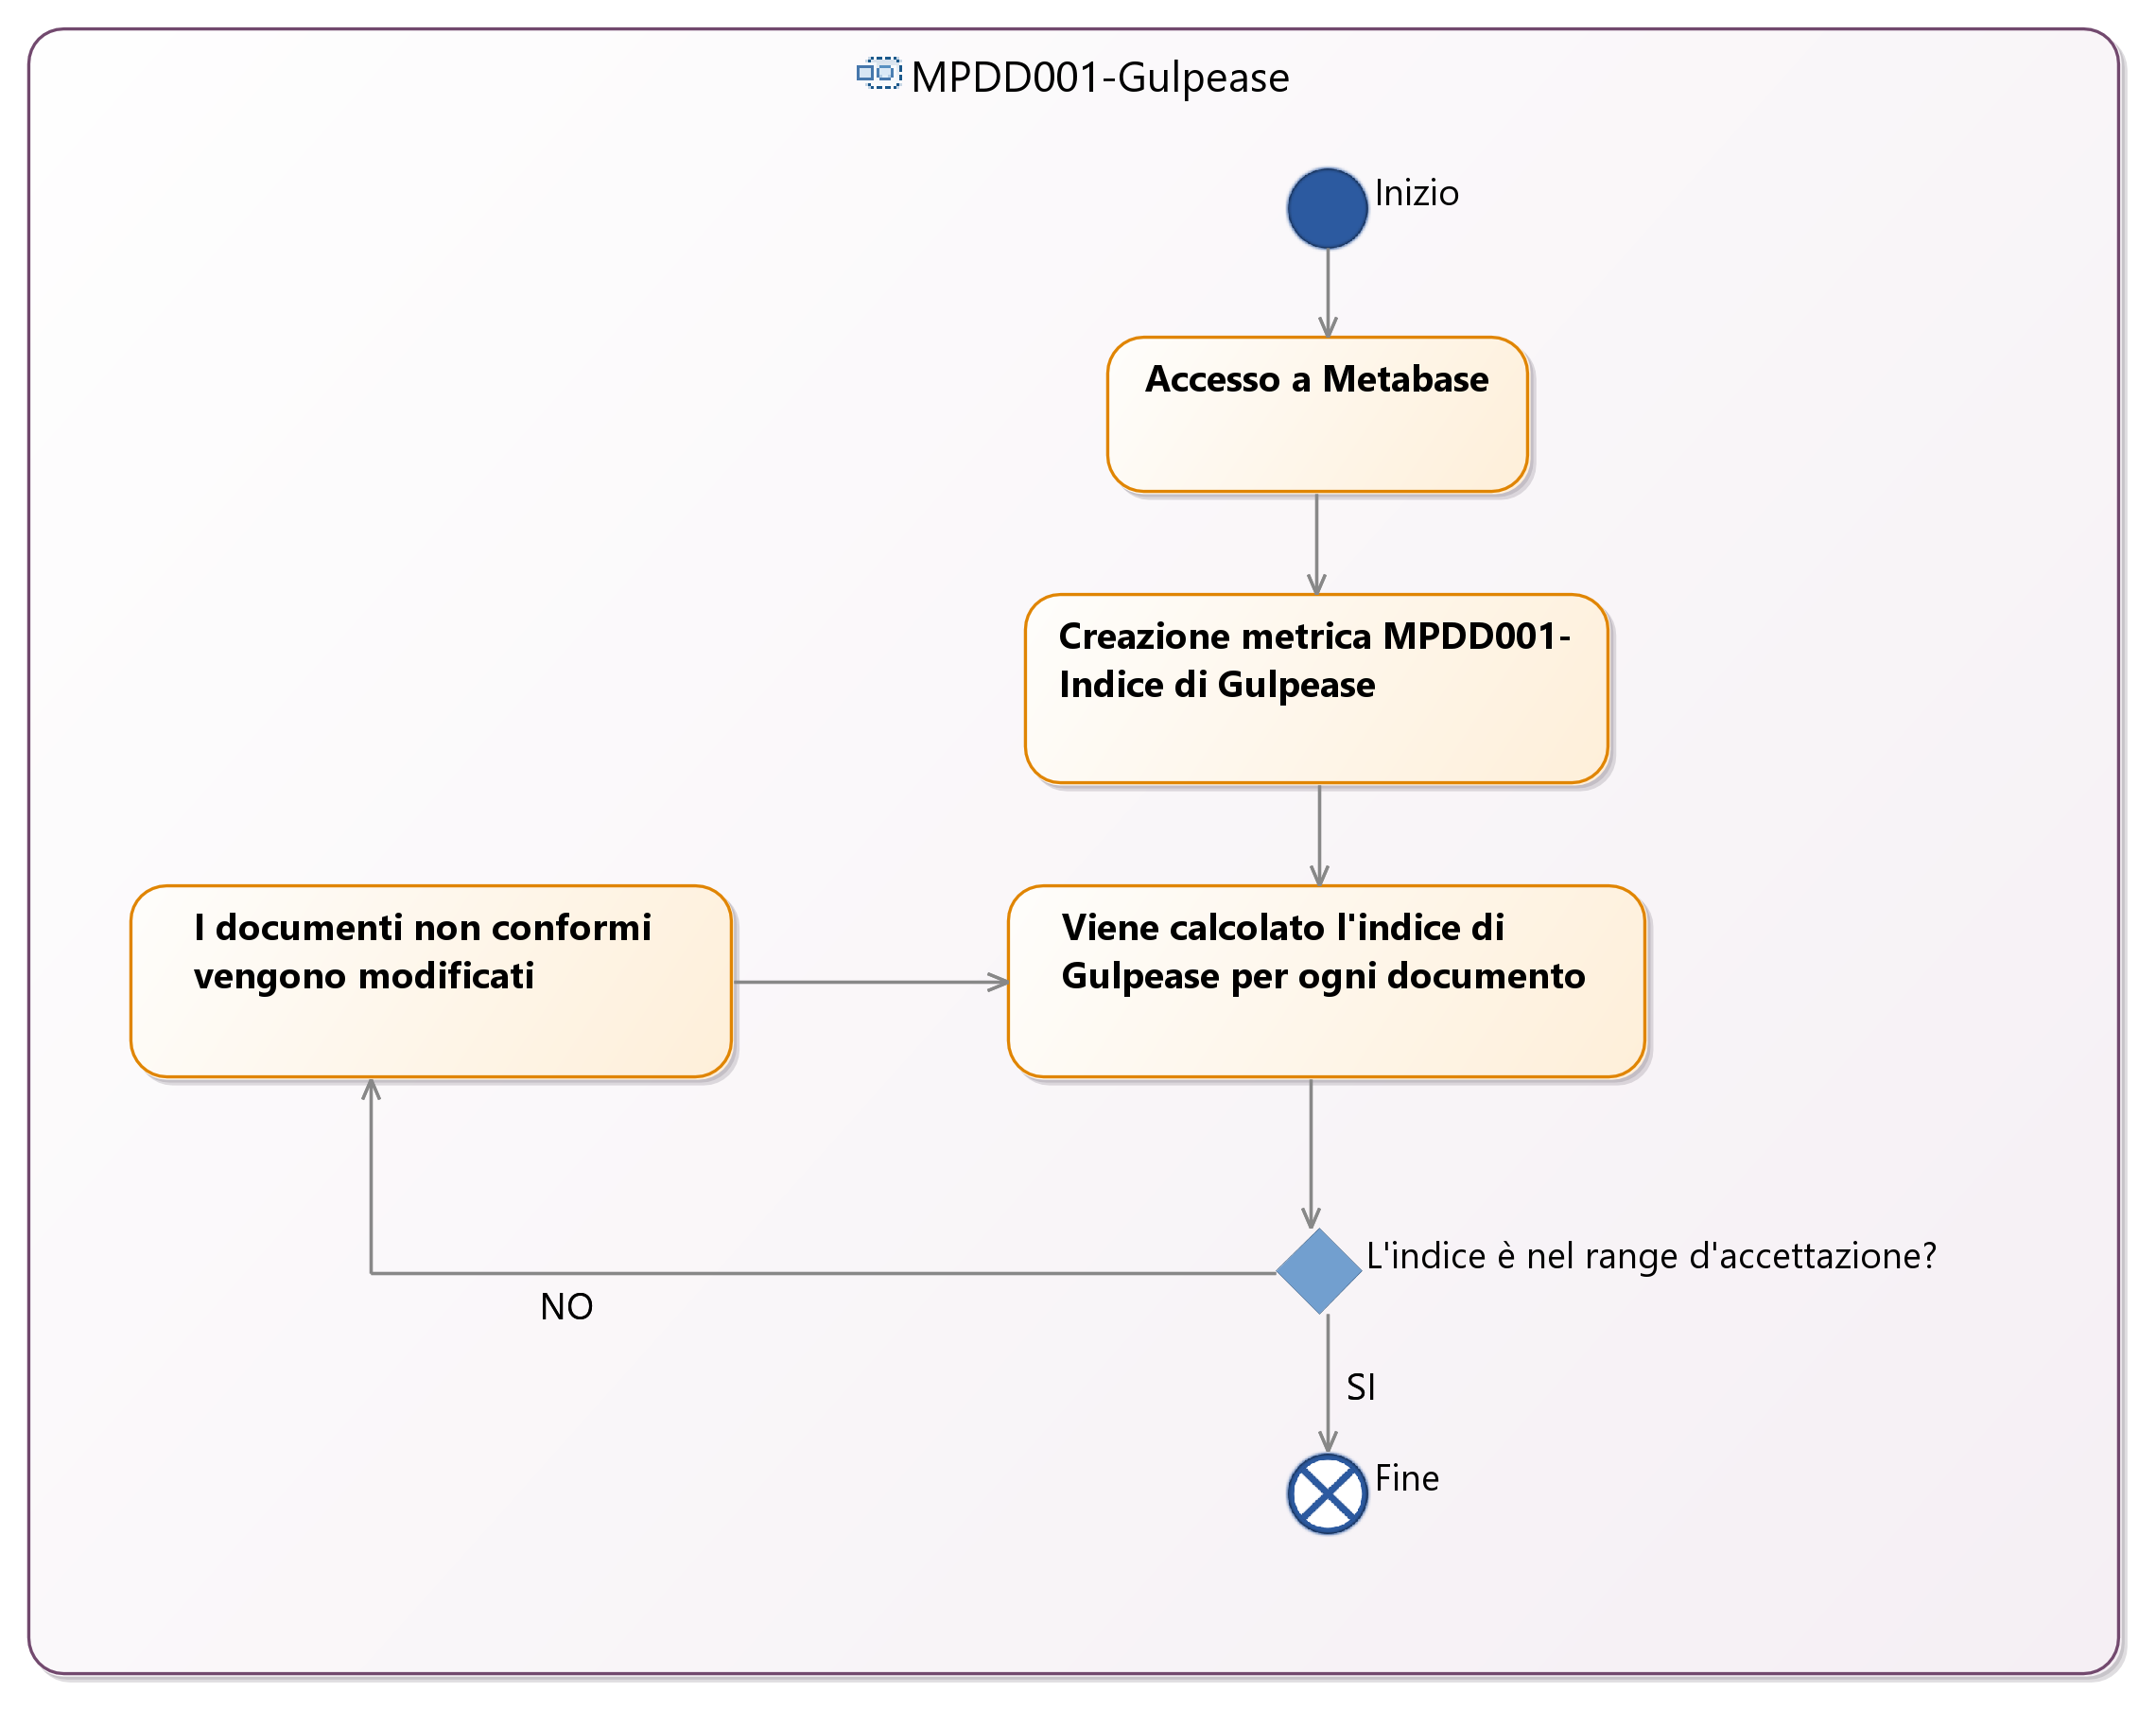
\includegraphics[scale=0.25]{../../common/images/MetricaGulpease}
	
	%VERI_GIORAT: errato il diagramma devi spiegare che ad ogni commit in automatico vengono inseriti valori gulpease su database. Quindi dopo inserimento automatico metabase realizza report aggiornato 
	
	 % calcolata tramite lo script "gulpease.py" citato nella sottosezione \textbf{Strumenti di supporto alla documentazione}.\\
	%L'implementazione di ulteriori metriche tramite procedure verrà studiato con l'avanzare del progetto.
	
	\section{Procedure di controllo di qualità di processo}
	La qualità dei processi verrà garantita dall'applicazione del metodo \citGloss{PDCA}, descritto dell'appendice A. Grazie a questo metodo sarà possibile ottenere un miglioramento continuo della qualità di tutti i processi, inclusa la \citGloss{verifica}, e come diretta conseguenza si otterrà il miglioramento dei prodotti risultanti.\\Per ottenere qualità dei processi, bisogna:
	\begin{itemize}
		\item \textbf{Definire il processo}: Affinché sia controllabile;
		\item \textbf{Controllare il processo}: In funzione dell'ottenimento di efficacia, efficienza ed esperienza;
		\item \textbf{Usare strumenti di valutazione}: SPICE e \citGloss{PDCA}.
	\end{itemize}

	\section{Configurazione}
	
	\subsection{Controllo di versione}
	
	\subsubsection{Descrizione}
	Per le parti versionabili del progetto e per i documenti ufficiali si è scelto l'utilizzo della tecnologia Git.
	La condivisione dei documenti informali e delle parti non versionabili è invece effettuata tramite l'uso di una cartella Google Drive condivisa.
	
	\subsubsection{Struttura delle repository}
	Sono state create due repository:
	\begin{itemize}
		\item \textquotedblleft Documentazione 353\textquotedblright, contenete i documenti ufficiali del progetto;
		\item \textquotedblleft PoC Marvin\textquotedblright, contenente il \poc sviluppato per la \tb.
	\end{itemize}
	
	I file interni al \citGloss{repository} \textquotedblleft Documentazione 353\textquotedblright\ sono organizzati secondo questa struttura:
	\begin{itemize}
		\item \textbf{Esterni:}
				\begin{itemize}
				\item \textbf{AnalisiDeiRequisiti};
				\item \textbf{Glossario};
				\item \textbf{PianoDiProgetto};
				\item \textbf{PianoDiQualifica};
				\item \textbf{Verbali esterni}.
			\end{itemize}
		\item \textbf{Interni:}
				\begin{itemize}
					\item \textbf{NormeDiProgetto};
					\item \textbf{Glossario};
					\item \textbf{StudioDiFattibilita};
					\item \textbf{Verbali interni}.
				\end{itemize}		
	\end{itemize}	
	All'interno di ogni cartella è stato definito un file \citGloss{LaTeX} principale che assume il nome del documento stesso ed il file \texttt{diariomodifiche.tex} per mantenere traccia delle modifiche effettuate.\\
	Nella root della \citGloss{repository} è stato messo invece un file \texttt{.sh} gestito tramite \citGloss{Travis} CI che controlla automaticamente gli errori in tutti i documenti presenti e compila un log con i risultati ottenuti.
	
	\subsubsection{Ciclo di vita dei branch}
	Per sfruttare il parallelismo nello sviluppo di uno stesso documento sono stati creati appositamente dei \citGloss{branch} denominati con il nome del membro o dei membri del gruppo che devono lavorare su una determinata parte, mentre i documenti baseline saranno invece contenuti nel master \citGloss{branch}.\\
	Il merge col master avviene quindi solamente quando un documento si trova in stato di "Approvato".
	
	\subsubsection{Aggiornamento della repository}
	Per l'aggiornamento della \citGloss{repository} è previsto il seguente sotto processo motivato dalla sezione precedente \textquotedblleft ciclo di vita":
	\begin{itemize}
		\item Verificare di trovarsi sul \citGloss{branch} personale con \textquotedblleft git branch"(quella selezionata presenta un asterisco *) e in caso di riscontro negativo cambiare branch con \textquotedblleft git checkout"
		\item Dare il comando \textquotedblleft git pull". Nel caso in cui si verifichino dei conflitti:
		\begin{itemize}
			\item Dare il comando \textquotedblleft git stash" per accantonare momentaneamente	le modifiche apportate;
			\item Dare il comando \textquotedblleft git pull" per ottenere ed applicare i \citGloss{commit} mancanti;
			\item Dare il comando \textquotedblleft git stash apply" per ripristinare le modifiche.
		\end{itemize}
		In questo modo il \citGloss{repository} locale risulta aggiornato rispetto il \citGloss{repository} remoto, mantenendo le modifiche personali apportate;
	
		\item Dare il comando \textquotedblleft git add [files]" , che aggiungerà i file modificati e quelli nuovi specificati;
		\item Dare il comando \textquotedblleft git commit" e successivamente riassumere le modifiche effettuate, in caso sia utile si può aggiungere un messaggio esteso di descrizione;
		\item Dare il comando \textquotedblleft git push" per completare l'operazione e fornire le modifiche agli altri membri del gruppo.
	\end{itemize}
	\subsection{Strumenti}
	\begin{itemize}
		\item \textbf{Client git:} verrano usati due client secondo le preferenze personali di ogni membro del gruppo tra Github Desktop\footnote{\nURI{https://desktop.github.com/}} e GitKraken\footnote{\nURI{https://www.gitkraken.com/}}, gratuito con licenza studenti;
		\item \textbf{Server git:} sarà utilizzato Github\footnote{\nURI{https://github.com/}} per affidabilità ed integrazione con strumenti esterni come \citGloss{Travis} facilitata. Era stato inoltre suggerito dal Referente oltre ad essere già utilizzato dalla maggior parte dei membri del gruppo.
	\end{itemize}

	
	\section{Verifica}
	
	\subsection{Descrizione}
	Un processo fondamentale per il proseguimento e l'evoluzione di un progetto è la \citGloss{verifica} su ogni suo sottoprodotto che porta alla creazione di un singolo componente.\\
	In questa sezione si descriveranno gli strumenti e i metodi che verranno usati per la \citGloss{verifica} del codice e dei documenti durante la loro realizzazione.\\
	Per quanto riguarda questa prima parte di progetto la \citGloss{verifica} si è concentrata essenzialmente su documenti e diagrammi.
	
	\subsection{Analisi statica}
	L'analisi statica è una tecnica di analisi applicabile sia alla documentazione che al codice e permette di effettuare la \citGloss{verifica} di quanto prodotto individuando errori ed anomalie.\\
	Essa può essere svolta in due modi diversi:
		\begin{itemize}
			\item \textbf{Walkthrough:} tecnica applicata quando non si sanno le tipologie di errori o problemi che si stanno cercando e quindi prevede una lettura da cima a fondo del codice o documento per trovare anomalie di qualsiasi tipo.\\
			Viene sempre svolto per la \citGloss{verifica} dei contenuti dei documenti;
						
			\item \textbf{Inspection:} tecnica da applicare quando si ha idea delle possibili problematiche che si stanno cercando e si attua leggendo in modo mirato il documento/codice sulla base di una lista di possibili errori precedentemente stilata.\\
			Viene realizzata tramite la checklist presente sul sito Todo353swe.
		\end{itemize}
	
	\subsection{Analisi dinamica}
	Il processo di analisi dinamica consiste nella realizzazione ed esecuzione di una serie di test sul codice del software di varie tipologie. Questa tecnica non è applicabile per trovare errori nella documentazione.
	
	\subsection{Verifica Diagrammi UML}
	I verificatori devono controllare tutti i diagrammi UML prodotti rispettino lo standard UML e che siano corretti semanticamente.
	
	\subsection{Strumenti}
	\begin{itemize}
		\item \textbf{Software:}
		sono stati scelti per la verifica Mocha e la libreria Chai per React, Redux e Solidity. Inoltre per verificare il codice in React viene utilizzato anche Enzyme;
		\item \textbf{Documenti:} per il controllo dei documenti prodotti utilizzeremo le funzionalità di TeXstudio assieme a script bash eseguiti automaticamente da \citGloss{Travis} per controllare che non ci siano errori nei file \citGloss{LaTeX}, per assicurarsi che il Glossario non presenti mancanze o duplicati e verificare l'assenza di errori ortografici;
		\item \textbf{Gestione processi e feedback:} è stato scelto di utilizzare il sistema integrato di issues\footnote{\nURI{https://guides.github.com/features/issues/}} presente su \citGloss{GitHub} per permettere un dialogo maggiore per ogni singola issue. 
		\item \textbf{Gestione tasklist:} Todo353swe\footnote{\nURI{https://todo353swe.netlify.com}} semplice sito per gestione tasklist realizzato dai membri del gruppo per utilizzo interno.
		\item \textbf{Analisi dinamica locale:} è stato scelto ESLint\footnote{\nURI{https://eslint.org/}} come soluzione iniziale per risolvere tutte le necessità di analisi del codice locale.
		\item \textbf{Analisi dinamica remota:} è stato individuato Sonarqube\footnote{\nURI{https://www.sonarqube.org/}} come soluzione iniziale da accertare, per risolvere tutte le necessità di analisi del codice del gruppo. Maggiori dettagli sarannò introdotti durante la creazione dei \poc per la Technology \citGloss{baseline}.
	\end{itemize}


	\section{Validazione}
	\subsection{Descrizione}
		Il processo di \citGloss{validazione} ha l'obiettivo di verificare che il prodotto sia conforme a quanto pianificato e sia abile nel gestire e minimizzare gli effetti degli errori.
	\subsection{Procedure}
		I passi per compiere l’attività di \citGloss{validazione} sono i seguenti:\\
		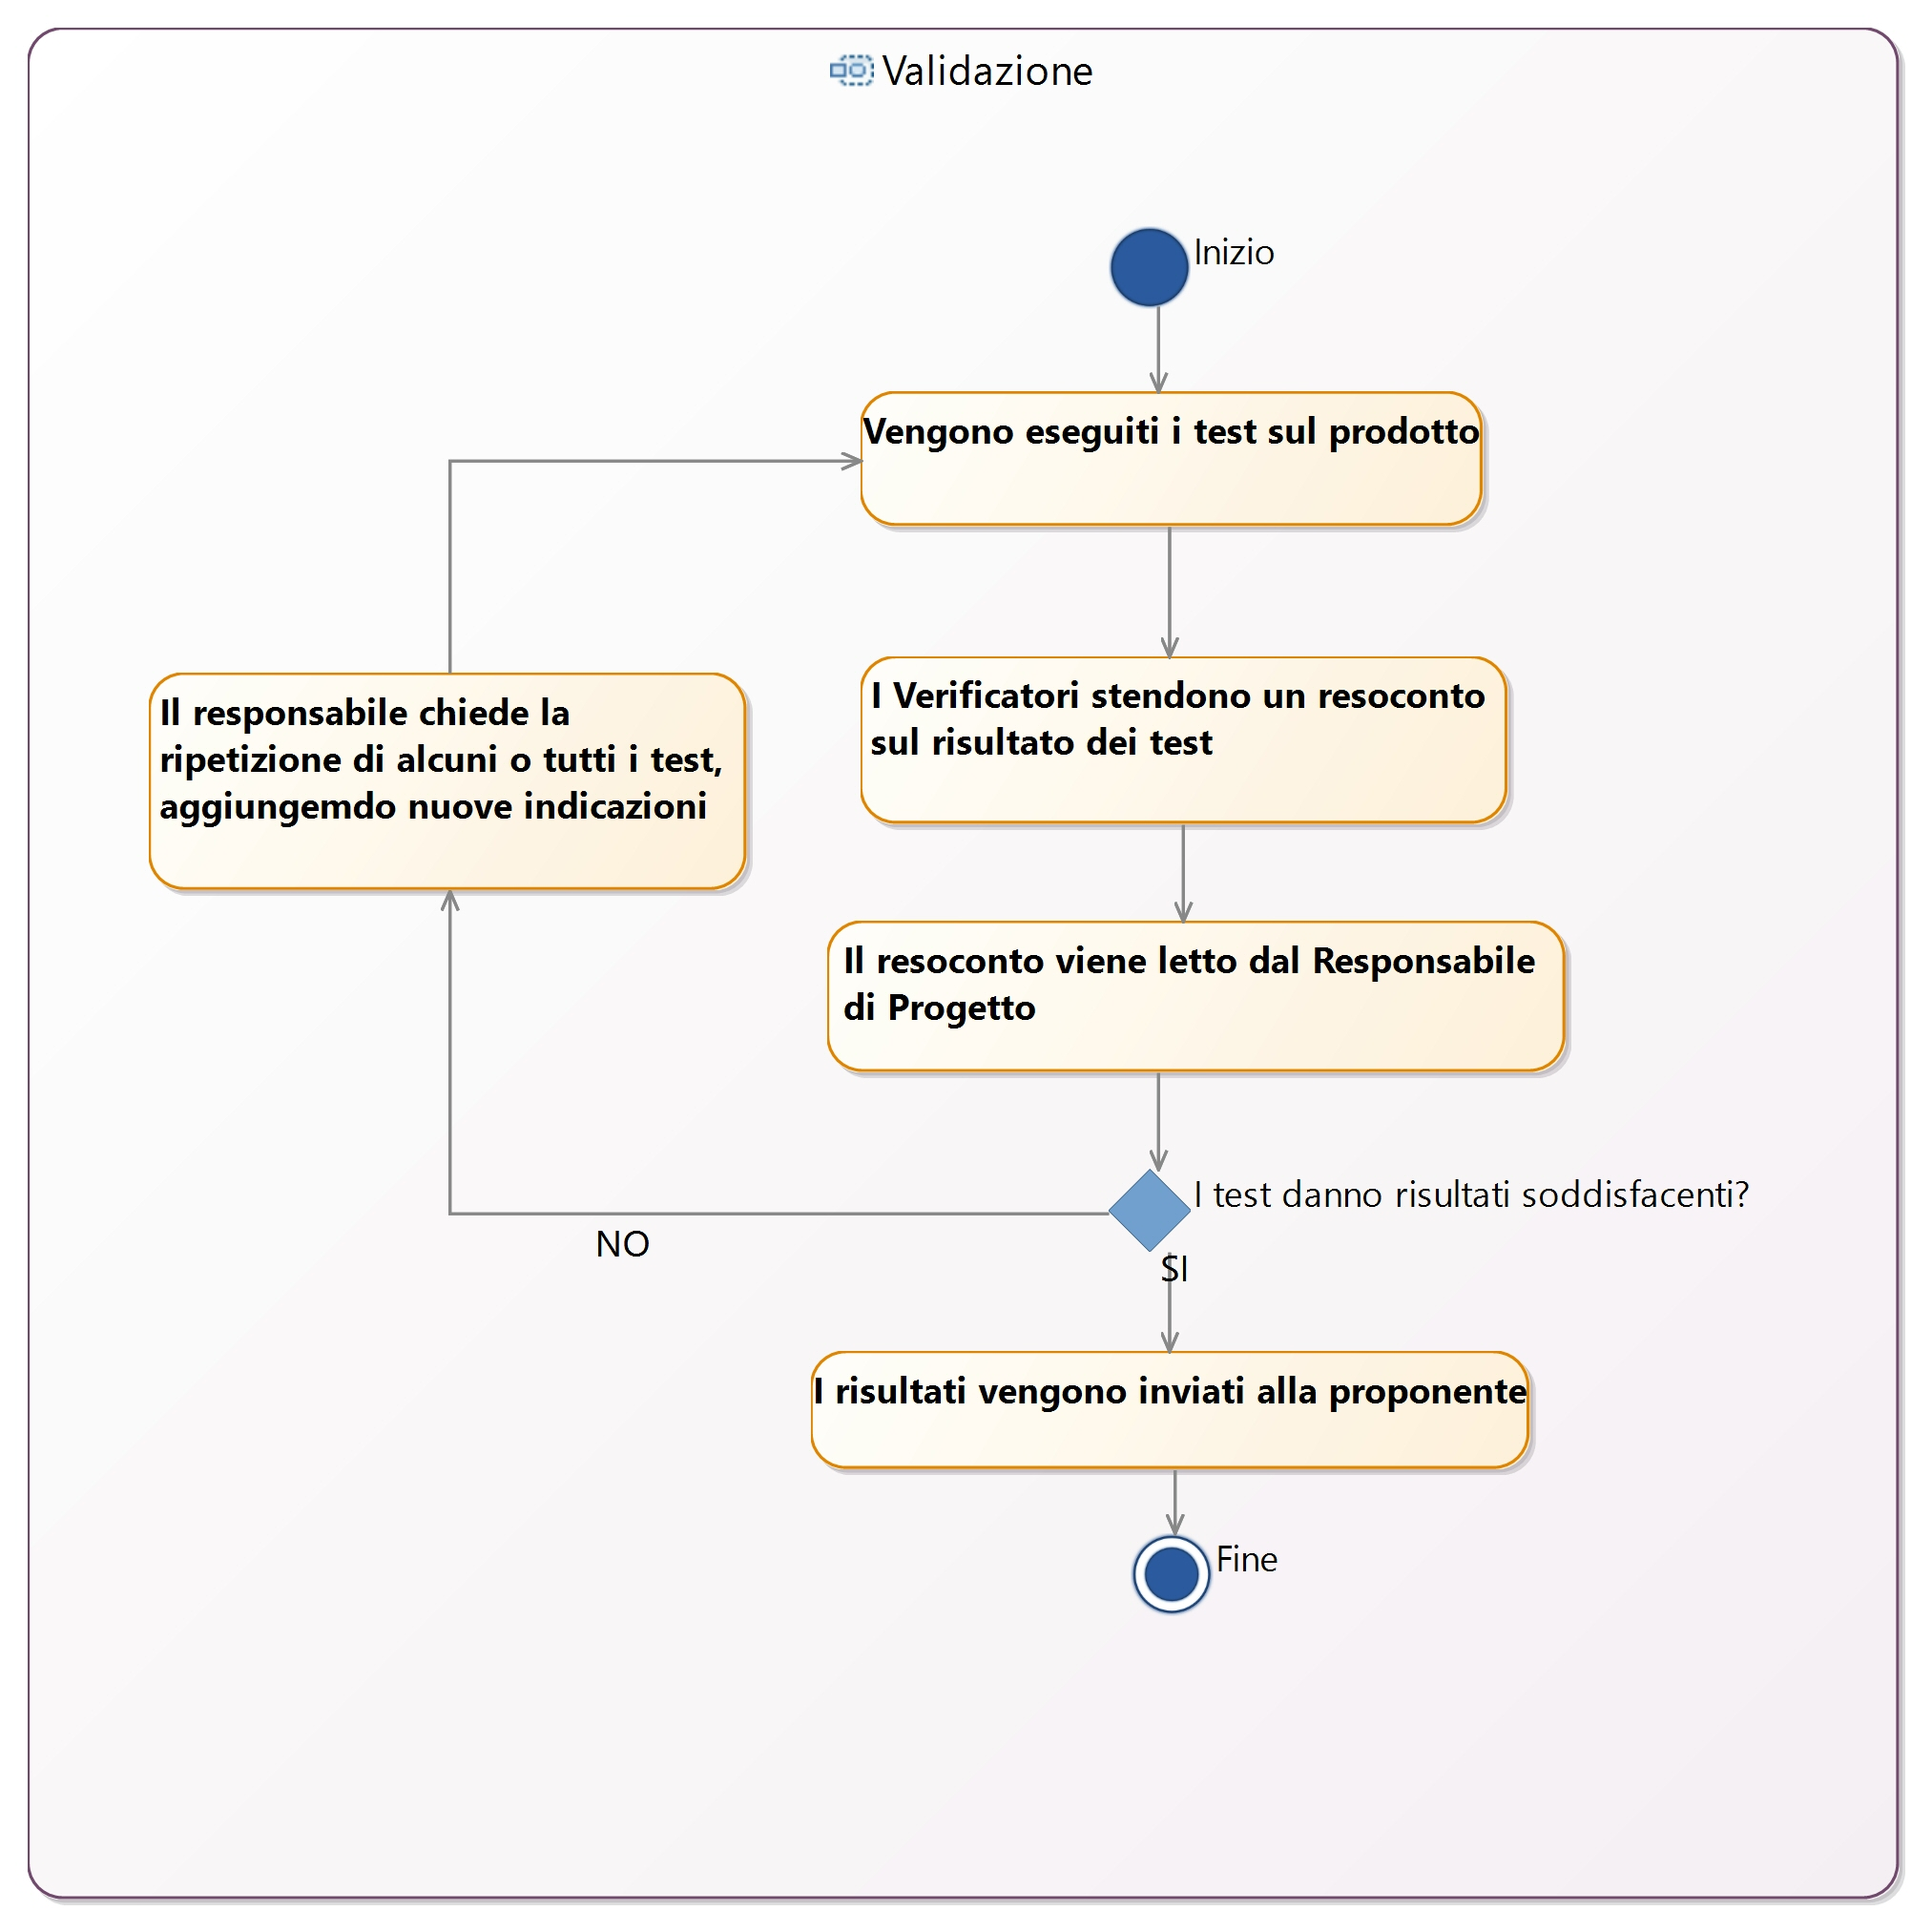
\includegraphics[scale=0.2]{../../common/images/Validation}

	 
	
	
\end{document}